\chapter{Particle-hole diagrams}
\label{chapter:particle-hole}

\section{Self-energy}
The particle-hole free-energy diagrams are given by
the following series:

\begin{center}
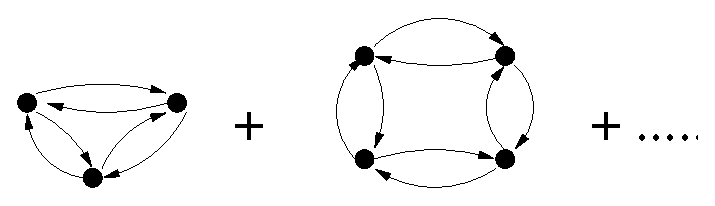
\epsfig{file=flex/phi_ph.eps}
\end{center}

Let $\chi^{ph}_{\nu_3\alpha_3 \nu_2 \alpha_2; 
\nu_1\alpha_1 \nu_0\alpha_0}(x_1,x_0)$ refer
to the following diagram:

\begin{center}
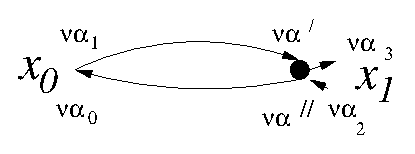
\epsfig{file=flex/chi_ph.eps}
\end{center}

Here $x$ refers to the space time label, $(\mathbf{r},\tau)$.
Mathematically, the above diagram is represented as
\begin{eqnarray}
\label{k_ph}
\chi^{ph}_{\nu_3\alpha_3 \nu_2 \alpha_2; \nu_1 \alpha_1 \nu_0\alpha_0}(x_1,x_0) 
& = & \frac{1}{2} \sum_{\nu^{\prime}\alpha^{\prime}\nu^{\prime\prime} \alpha^{\prime\prime}}
\Gamma^{(0)ph}_{\nu_3\alpha_3\nu_2\alpha_2; 
\nu^{\prime}\alpha^{\prime}\nu^{\prime\prime}\alpha^{\prime\prime}}\,
G_{\nu^{\prime}\alpha^{\prime}\nu_1 \alpha_1}(x_1,x_0) \; G_{\nu_0\alpha_0 
\nu^{\prime\prime}\alpha^{\prime\prime}}(x_0,x_1) \\
& = & -\frac{1}{2}\sum_{\nu^{\prime}\alpha^{\prime}\nu^{\prime\prime} \alpha^{\prime\prime}} 
\Gamma^{(0)ph}_{\nu_3\alpha_3 \nu_2 \alpha_2; \nu^{\prime}\alpha^{\prime}
\nu^{\prime\prime}\alpha^{\prime\prime}}\,
\tilde{\chi}^{ph}_{\nu^{\prime}\alpha^{\prime}\nu^{\prime\prime} \alpha^{\prime\prime}; 
\nu_1\alpha_1\nu_0\alpha_0 \beta_0}(x_1,x_0)
\end{eqnarray}
where
\begin{equation}
\label{chi_ph}
\tilde{\chi}^{ph}_{\nu^{\prime}\alpha^{\prime}\nu^{\prime\prime}\alpha^{\prime\prime}; 
\nu_1\alpha_1 \nu_0\alpha_0}(x_1,x_0) \equiv
(-1) G_{\nu^{\prime}\alpha^{\prime}\nu_1 \alpha_1}(x_1,x_0) \; 
G_{\nu_0\alpha_0 \nu^{\prime\prime}\alpha^{\prime\prime}}(x_0,x_1)
\end{equation}
and
\begin{equation}
\Gamma^{(0),ph}_{\alpha_1 \beta_1; \alpha^{\prime}\beta^{\prime}} \equiv
- \Gamma^{(0)}_{\alpha_1 \beta^{\prime}; \beta_1 \alpha^{\prime}}.
\end{equation}
The overall positive sign comes from two factors of (-1):
one from a closed fermion loop and one from the vertex.

Graphically, the particle-hole vertex is obtained from
the standard form of the four-point vertex 
as follows:
\begin{center}
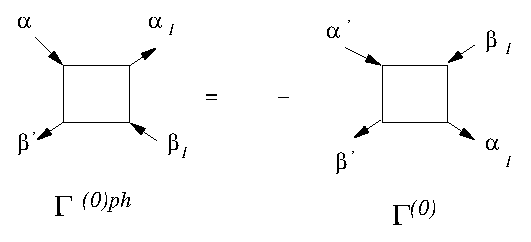
\epsfig{file=flex/ph_vertex.eps}
\end{center}
and the minus sign is seen to emerge from the exchange of labels
on the right side of the vertex.

For a translationally invariant system we have
\begin{equation}
\tilde{\chi}^{ph}_{\alpha^{\prime}\beta^{\prime}; 
\alpha_0 \beta_0}(\tau,\mathbf{r}) \equiv
(-1) G_{\alpha^{\prime} \alpha_0}(\tau,\mathbf{r}) \; 
G_{\beta_0 \beta^{\prime}}(-\tau,-\mathbf{r})
\end{equation}
It is convenient to combine $\alpha^{\prime}\beta^{\prime}$
into a single index, $\nu^{\prime} \equiv
4 \alpha^{\prime} + \beta^{\prime}$ with the same
for $\alpha_0\beta_0$.  We then have
\begin{equation}
\tilde{\chi}^{ph}_{\nu^{\prime},\nu_0}(\tau,\mathbf{r}) \equiv
\tilde{\chi}^{ph}_{\alpha^{\prime}\beta^{\prime}; 
\alpha_0 \beta_0}(\tau,\mathbf{r})
\end{equation}
The same can be done for $\Gamma^{(0)ph}$ such that
\begin{equation}
\chi^{ph}_{\alpha_1\beta_1,\alpha_0\beta_0}(\tau,\mathbf{r}) 
=-\frac{1}{2} \sum_{\alpha^{\prime}\beta^{\prime}} 
\Gamma^{(0)ph}_{\alpha_1\beta_1;\alpha^{\prime}\beta^{\prime}}
\tilde{\chi}^{ph}_{\alpha^{\prime}\beta^{\prime};\alpha_0\beta_0}
(\tau,\mathbf{r})
\end{equation}
can be interpretted as a simple matrix equation for each combination
of $\tau$ and $\mathbf{r}$ values:
\begin{equation}
\left[\chi^{ph}(\tau,\mathbf{r})\right]_{\nu_1,\nu_0} =
-\frac{1}{2}\left[\Gamma^{(0)}\,\tilde{\chi}^{ph}(\tau,\mathbf{r})\right]_{\nu_1,\nu_0}
\end{equation}
where $\chi^{ph}$, $\Gamma^{(0)ph}$, and $\tilde{\chi}^{ph}$
are taken as $16 \times 16$ matrices using the indexing scheme
described above.

This simplifies the representation of $\Phi_{ph}$.  For
example, we can write
\begin{equation}
\Phi_{ph}^{n=3} = - \frac{T}{3}
\sum_{\alpha_i \beta_i}
\int dx_0 \,dx_1 \, dx_2 \;
\chi^{ph}_{\alpha_2 \beta_2; \alpha_1 \beta_1}(x_2,x_1)
\chi^{ph}_{\alpha_1 \beta_1; \alpha_0 \beta_0}(x_1,x_0)
\chi^{ph}_{\alpha_0 \beta_0; \alpha_2 \beta_2}(x_0,x_2).
\end{equation}
On account of space and time invariance, we can write
\begin{equation}
\chi^{ph}_{\alpha_i \beta_i; \alpha_j \beta_j}(x_i, x_j) =
\frac{T}{N} \sum_{\omega_m \mathbf{q}}
e^{-i \omega_m(\tau_i - \tau_j) + 
i \mathbf{q}\cdot(\mathbf{r}_i - \mathbf{r}_j)} \;
\chi^{ph}_{\alpha_i \beta_i; \alpha_j \beta_j}(\omega_m,\mathbf{q}).
\end{equation}
On subsitution we get
\begin{eqnarray}
\Phi_{ph}^{n=3} & = & - \frac{T}{3}
\sum_{\alpha_i \beta_i}
\sum_{\omega_m \mathbf{q}}
\chi^{ph}_{\alpha_2 \beta_2; \alpha_1 \beta_1}(\omega_m, \mathbf{q})
\chi^{ph}_{\alpha_1 \beta_1; \alpha_0 \beta_0}(\omega_m, \mathbf{q})
\chi^{ph}_{\alpha_0 \beta_0; \alpha_2 \beta_2}(\omega_m, \mathbf{q})
\\
& = & - \frac{T}{3} \sum_{\omega_m \mathbf{q}} 
\mathrm{Tr} \; (\chi^{ph}(\omega_m, \mathbf{q}))^3.
\end{eqnarray}
Summing over all orders then,  we have
\begin{eqnarray}
\Phi_{ph} = -T \sum_{n > 2} \frac{1}{n}
\; \mathrm{Tr} \; (\chi^{ph})^n
\end{eqnarray}
where the trace, $\mathrm{Tr}$, runs over frequency, momenta,
and the spin indices of the products of the $16 \times 16$
matrix $\chi^{ph}$.

The self-energy is obtained by functional differention
of $\Phi_{ph}$ with the $n^{th}$-order particle-hole self-energy
given by
\begin{equation}
\label{sigma_ph1}
\begin{split}
\Sigma^{ph,n}_{\alpha \alpha^{\prime}}(x,x^{\prime}) & = 
T \frac{\delta\; \Phi_{ph}^n}
{\delta\; G_{\alpha^{\prime} \alpha}(x^{\prime},x)} \\
\\
& = -T^{2} \sum_{\alpha_i \beta_i}
 \int dx_0 \cdots dx_{n-1} \,
 \chi^{ph}_{\alpha_0 \beta_0; \alpha_{n-1} \beta_{n-1}}(x_0, x_{n-1}) 
 \cdots \\
& \quad \quad \quad \frac{\delta   
 \chi^{ph}_{\alpha_j \beta_j; \alpha_{j-1} \beta_{j-1}}(x_j, x_{j-1})}
 {\delta G_{\alpha^{\prime} \alpha}(x^{\prime},x)}
 \cdots
 \chi^{ph}_{\alpha_1 \beta_1; \alpha_0 \beta_0}(x_1,x_0) 
\end{split}
\end{equation}
Using the definition of $\chi^{ph}$ from Eq.~(\ref{k_ph}) we
get
\begin{equation}
\label{deriv_kph}
\begin{split}
\frac{\delta\; \chi_{\alpha_j \beta_j; \alpha_{j-1} \beta_{j-1}}(x_j, x_{j-1})}
{\delta G_{\alpha^{\prime} \alpha}(x^{\prime},x)} & = 
\frac{1}{2} \sum_{\gamma_j \delta_j} 
        \Gamma^{(0),ph}_{ \alpha_j \beta_j;\gamma_j\delta_j}
 \delta_{\gamma_j,\alpha^{\prime}}
                           \delta_{\alpha_{j-1},\alpha}
  \frac{ \delta(x_j - x^{\prime})}{T}\,
 \frac{\delta(x_{j-1} - x)}{T}
                           G_{\beta_{j-1}\delta_j}(x_{j-1},x_j) 
\\
& \quad + 
 \Gamma^{(0),ph}_{ \alpha_j \beta_j;\gamma_j\delta_j}
G_{\gamma_j \alpha_{j-1}}(x_j,x_{j-1})
                          \delta_{\beta_{j-1},\alpha^{\prime}}
                          \delta_{\delta_j,\alpha}
             \frac{\delta(x_{j-1} - x^{\prime})}{T}\,
                     \frac{\delta(x_j - x)}{T}
 \\
= &  \frac{1}{2\, T^2}
\sum_{\delta_j} 
 \Gamma^{(0),ph}_{\alpha_j \beta_j; \alpha^{\prime}\delta_j}
\delta_{\alpha_{j-1},\alpha} 
                      \delta(x_j - x^{\prime})
                      \delta(x_{j-1} - x) G_{\beta_{j-1}\delta_j}(x,x^{\prime})
\\
& + \frac{1}{2\, T^2}
\sum_{\gamma_j} 
 \Gamma^{(0),ph}_{\alpha_j\beta_j; \gamma_j \alpha }
\delta_{\beta_{j-1},\alpha^{\prime}}
                    \delta(x_{j-1} - x^{\prime}) 
                    \delta(x_j - x)
                    G_{\gamma_j \alpha_{j-1}}(x,x^{\prime})
\end{split}
\end{equation}
Substitution of Eq.~(\ref{deriv_kph}) into Eq.~(\ref{sigma_ph1})
yields
\begin{equation}
\begin{split}
\Sigma^{ph,n}_{\alpha \alpha^{\prime}}(x,x^{\prime})
=&- \frac{1}{2} \sum_{\alpha_i \beta_i} \int dx_0 \cdots dx_{n-1} \cdots
 \chi^{ph}_{\alpha_{j+1} \beta_{j+1},\alpha_j \beta_j}(x_{j+1},x_j) \\
& \big( \sum_{\delta_j} 
\Gamma^{(0),ph}_{\alpha_j \beta_j;\alpha^{\prime}\delta_j} 
\delta_{\alpha_{j-1},\alpha}
\delta(x_j - x^{\prime}) \delta(x_{j-1}-x) 
G_{\beta_{j-1}\delta_j}(x,x^{\prime}) 
\\
& + \sum_{\gamma_j}
\Gamma^{(0),ph}_{\alpha_j \beta_j;\gamma_j\alpha}
 \delta_{\beta_{j-1},\alpha^{\prime}}
\delta(x_{j-1} - x^{\prime}) \delta(x_j - x)
G_{\gamma_j \alpha_{j-1}}(x,x^{\prime})
 \big)
\\
& \chi^{ph}_{\alpha_{j-1} \beta_{j-1}; \alpha_{j-2}\beta_{j-2}}(x_{j-1},
x_{j-2}) \cdots
\end{split}
\end{equation}
It can be shown that the each of the terms within the parenthesis
produces an equivalent result after all sums
and integrations are performed.  This equivalence is
expected as one obtains an equivalent self-energy
diagram regardless of which of the two Green's functions
is broken in a particle hole pair.
Consequently, we are able to double the first term
in the parenthesis and ignore the second.

Using the above simplification and integrating and summing over
$\delta$-functions produces
\begin{equation}
\begin{split}
\Sigma^{ph,n}_{\alpha \alpha^{\prime}}(x,x^{\prime})
= &  \; - \sum_{\alpha_i \beta_i, \delta_j, !\alpha_{j-1}}
\int dx_0 \cdots dx_{j-2} dx_{j+1} \cdots dx_{n-1} \cdots
\\
& \chi^{ph}_{\alpha_{j+1}\beta_{j+1}; \alpha_j \beta_j}(x_{j+1},x^{\prime})
\Gamma^{(0),ph}_{\alpha_j \beta_j;\alpha^{\prime}\delta_j}
G_{\beta_{j-1}\delta_j}(x,x^{\prime}) 
\\
& \chi^{ph}_{\alpha \beta_{j-1}; \alpha_{j-2} \beta_{j-2}}(x,x_{j-2}) \cdots
\end{split}
\end{equation}
The spin sum does not include $\alpha_{j-1}$.
However, we substitute the dummy index $\alpha_{j-1}$
for the dummy index $\delta_j$, giving us
\begin{equation}
\begin{split}
\Sigma^{ph,n}_{\alpha \alpha^{\prime}}(x,x^{\prime})
= & - \sum_{\alpha_i \beta_i} 
\int dx_0 \cdots dx_{j-2} dx_{j+1} \cdots dx_{n-1} \cdots
\\
& \chi^{ph}_{\alpha_{j+1} \beta_{j+1}; \alpha_j \beta_j}(x_{j+1},x^{\prime})
\;
\Gamma^{(0),ph}_{\alpha_j \beta_j; \alpha^{\prime} \alpha_{j-1}}
 G_{\beta_{j-1}\alpha_{j-1}}(x,x^{\prime})
\\
& 
\chi^{ph}_{\alpha \beta_{j-1}; \alpha_{j-2} \beta_{j-2}}(x, x_{j-2}) \cdots 
\end{split}
\end{equation}
For convenience, we relabel the dummy indices:
$j - 1 \to 0$, $j \to 1$, $j + 1 \to 2$, $\cdots$,
$j - 2 \to n-1$.  We get
\begin{equation}
\begin{split}
\Sigma^{ph,n}_{\alpha \alpha^{\prime}}(x,x^{\prime})
= & - \sum_{\alpha_i \beta_i} 
\int dx_2 dx_3 \cdots dx_{n-1} \cdots
\\
& \chi^{ph}_{\alpha_2 \beta_2; \alpha_1 \beta_1}(x_2,x^{\prime})
\;
\Gamma^{(0)ph}_{\alpha_1 \beta_1; \alpha^{\prime} \alpha_0}
 G_{\beta_0\alpha_0}(x,x^{\prime})
\\
& 
\chi^{ph}_{\alpha \beta_0; \alpha_{n-1} \beta_{n-1}}(x, x_{n-1}) \cdots 
\end{split}
\end{equation}
Rewriting the above
we get
\begin{equation}
\begin{split}
\Sigma^{ph,n}_{\alpha\alpha^{\prime}}(x,x^{\prime}) = &
-\sum_{\alpha_0\beta_0} G_{\beta_0 \alpha_0}(x,x^{\prime}) \;
 \sum_{\alpha_1 \beta_1} \big( \prod_{i \geq 2}^{n-1} \int dx_i \sum_{\alpha_i \beta_i} \big)
\Gamma^{(0)ph}_{\alpha_1 \beta_1; \alpha^{\prime}\alpha_0}
\chi^{ph}_{\alpha_2 \beta_2; \alpha_1 \beta_1}(x_2, x^{\prime})
\\
& \chi^{ph}_{\alpha_3 \beta_3; \alpha_2 \beta_2}(x_3, x_2)
\cdots
\chi^{ph}_{\alpha \beta_0; \alpha_{n-1} \beta_{n-1}}(x,x_{n-1}) \\
= & - \sum_{\alpha_0\beta_0} G_{\beta_0 \alpha_0}(x,x^{\prime}) \;
 \sum_{\alpha_1 \beta_1}
 \big( \prod_{i \ge 2}^{n-1} \int dx_i \sum_{\alpha_i \beta_i} \big) 
 \chi^{ph}_{\alpha \beta_0; \alpha_{n-1} \beta_{n-1}}(x,x_{n-1})
\\
& \chi^{ph}_{\alpha_{n-1} \beta_{n-1}; \alpha_{n-2} \beta_{n-2}}(x_{n-1},x_{n-2})
\cdots \chi_{\alpha_2\beta_2; \alpha_1 \beta_1}(x_2, x^{\prime})
\Gamma^{(0)ph}_{\alpha_1 \beta_1; \alpha^{\prime}\alpha_0}
\end{split}
\end{equation}
The overall minus sign for each term is due to having either
an odd number of vertices and even number of closed loops or
the opposite.

We define 
\begin{equation}
\begin{split}
T^{ph,n}_{\alpha\beta_0; \alpha^{\prime}\alpha_0}(x,x^{\prime}) =
& \;
 \sum_{\alpha_1 \beta_1} \big( \prod_{i \ge 2}^{n-1} 
\int dx_i \sum_{\alpha_i \beta_i} \big) 
\chi^{ph}_{\alpha \beta_0; \alpha_{n-1} \beta_{n-1}}(x,x_{n-1})
\\ &
\chi^{ph}_{\alpha_{n-1} \beta_{n-1}; \alpha_{n-2} \beta_{n-2}}(x_{n-1},x_{n-2})
\cdots \chi_{\alpha_2\beta_2; \alpha_1 \beta_1}(x_2, x^{\prime})
\Gamma^{(0)ph}_{\alpha_1 \beta_1; \alpha^{\prime}\alpha_0}
\end{split}
\end{equation}
so that
\begin{equation}
\Sigma^{ph,n}_{\alpha\alpha^{\prime}}(x,x^{\prime}) =
-\sum_{\alpha_0 \beta_0}
G_{\beta_0 \alpha_0}(x,x^{\prime})\; 
T^{ph,n}_{\alpha \beta_0; \alpha^{\prime} \alpha_0}(x,x^{\prime})
\end{equation}

\section{$T$-matrix}

The Fourier transform of $T^{ph,n}$ is defined by
\begin{equation}
T^{ph,n}_{\alpha \beta_0; \alpha^{\prime} \alpha_0}(\omega_m,\mathbf{q})
\equiv \int_0^{\beta} d\tau \sum_{\mathbf{r}}
e^{i \omega_m (\tau - \tau^{\prime})
- i\mathbf{q}\cdot(\mathbf{r}-\mathbf{r}^{\prime})}\;
T^{ph}_{\alpha \beta_0; \alpha^{\prime}\alpha_0}(x, x^{\prime}).
\end{equation}
After expressing $T^{ph}$ in terms of $\chi^{ph}$ we get
\begin{equation}
\begin{split}
T^{ph,n}_{\alpha \beta_0; \alpha^{\prime}\alpha_0}(\omega_m,\mathbf{q})
= & \frac{T^{n-1}}{N^{n-1}}
\big( \prod_{i \geq 1}^{n-1} \sum_{\alpha_i \beta_i} \big)
\int dx dx_2 \cdots dx_{n-1}
e^{i \omega_m (\tau - \tau^{\prime}) 
-i \mathbf{q} \cdot (\mathbf{r} - \mathbf{r}^{\prime})} \\
& \sum_{w_{m_{n-1}} \mathbf{q}_{n-1}}
e^{-i \omega_{m_{n-1}}(\tau - \tau_{n-1})
+i \mathbf{q}_{n-1} \cdot (\mathbf{r} - \mathbf{r}_{n-1})}
\chi^{ph}_{\alpha \beta_0; \alpha_{n-1} \beta_{n-1}}(\omega_{m_{n-1}},
\mathbf{q}_{n-1}) \cdots \\
& \sum_{\omega_{m_1},\mathbf{q}_1} 
e^{-i \omega_{m_1}(\tau_2 - \tau^{\prime})+
i \mathbf{q}_1 \cdot (\mathbf{r}_2 - \mathbf{r}^{\prime})}
\chi^{ph}_{\alpha_2 \beta_2; \alpha_1 \beta_1}(\omega_{m_1},\mathbf{q}_1)
\Gamma^{(0)ph}_{\alpha_1 \beta_1; \alpha^{\prime}\alpha_0}
\\ \\
= &  
\big( \prod_{i \geq 1}^{n-1} \sum_{\alpha_i \beta_i} \big)
\chi^{ph}_{\alpha \beta_0; \alpha_{n-1}\beta_{n-1}}(\omega_m, \mathbf{q})
\cdots \chi^{ph}_{\alpha_2 \beta_2; \alpha_1 \beta_1}
(\omega_m, \mathbf{q}) 
\Gamma^{(0)ph}_{\alpha_1 \beta_1; \alpha^{\prime}\alpha_0} \\
= &  \left[ \left(\chi^{ph}(\omega_m,\mathbf{q})\right)^{n-1}
\mathbf{\Gamma}^{(0)ph} \right]_{\alpha \beta_0; \alpha^{\prime}\alpha_0}
\end{split}
\end{equation}

Since
\begin{equation}
\mathbf{T}^{ph} = \sum_{n \geq 3} 
\mathbf{T}^{ph,n}
\end{equation}
we have
\begin{eqnarray}
\mathbf{T}^{ph} & = & \sum_{n \geq 3} (\chi^{ph})^{n-1}
\mathbf{\Gamma}^{(0)ph} \\
& = &  (\sum_{n \geq 0} 
(\chi^{ph})^{n} - (\mathbf{I} + \chi^{ph}))
\mathbf{\Gamma}^{(0)ph} \\
& = &  ( (\mathbf{I} - \chi^{ph})^{-1} - (\mathbf{I}
+ \chi^{ph})) \mathbf{\Gamma}^{(0)ph} \\
& = &  ( (\mathbf{I} - (\mathbf{I}+\chi^{ph})
(\mathbf{I} - \chi^{ph}))(\mathbf{I} - \chi^{ph})^{-1}
\mathbf{\Gamma}^{(0)ph} \\
& = &  (\chi^{ph})^2 (\mathbf{I} - \chi^{ph})^{-1}
\mathbf{\Gamma}^{(0)ph}
\end{eqnarray}

It is also possible to include the second-order self-energy by
adding an extra term.  In that case, we get
\begin{equation}
\label{tph_def}
\mathbf{T}^{ph} = \left[\frac{\chi^{ph}}{2} +  
(\chi^{ph})^2 (\mathbf{I} - \chi^{ph})^{-1} \right]
\mathbf{\Gamma}^{(0)ph}
\end{equation}
where the factor of two is needed to avoid overcounting the
second-order self-energy diagram.

\section{Asymptotics}
The large frequency asymptotic behavior for $\chi^{ph}$ and
$T^{ph}$ can be traced to the same
for $\tilde{\chi}^{ph}$ which is defined in Eq.~(\ref{chi_ph}).
We have 
\begin{eqnarray}
\Delta \tilde{\chi}(\mathbf{r}) & \equiv &
\tilde{\chi}(\tau \to 0^+,\mathbf{r}) -
\tilde{\chi}(\tau \to 0^-,\mathbf{r}) \\
\Delta \tilde{\chi}^{\prime}(\mathbf{r}) & \equiv &
\tilde{\chi}^{\prime}(\tau \to 0^+,\mathbf{r}) -
\tilde{\chi}^{\prime}(\tau \to 0^-,\mathbf{r}).  
\end{eqnarray}
For each value of $\mathbf{r}$ these discontinuities are 
$16 \times 16$ matrices.
We get the discontinuities for $\chi$ using ordinary 
matrix multiplication:
\begin{eqnarray}
\Delta \chi^{ph}(\mathbf{r}) & = &
-\frac{1}{2} \mathbf{\Gamma}^{(0)ph}\;\Delta \tilde{\chi}(\mathbf{r}) \\
\Delta \chi^{ph \prime}(\mathbf{r}) & = &
-\frac{1}{2}\mathbf{\Gamma}^{(0)ph}\;\Delta \tilde{\chi}^{\prime}(\mathbf{r}) 
\end{eqnarray}
In the large frequency limit, we have
\begin{equation}
\label{kph_asy}
\lim_{|\omega_m| \to \infty}
\chi^{ph}(\omega_m, \mathbf{q})
= - \frac{\Delta \chi^{ph}(\mathbf{q})}{i \omega_m}
+ \frac{\Delta \chi^{ph \prime}(\mathbf{q})}{(i \omega_m)^2}
+ O \left( \frac{1}{(i \omega_m)^3} \right)
\end{equation}
where the discontinuities in $\mathbf{q}$-space for
$\chi^{ph}$ are obtained from a simple Fourier transform
of the discontinuities in $\mathbf{r}$-space, \textit{i.e.}
\begin{equation}
\Delta \chi^{ph}(\mathbf{q}) = \sum_{\mathbf{r}}
e^{-i \mathbf{q}\cdot\mathbf{r}}\Delta \chi^{ph}(\mathbf{r}).
\end{equation} 

Substitution of Eq.~(\ref{kph_asy}) into
Eq.~(\ref{tph_def}) yields an asymptotic expression
for $\mathbf{T}^{ph}$:
\begin{equation}
\begin{split}
\lim_{|\omega_m| \to \infty}
\mathbf{T}^{ph}(\omega_m,\mathbf{q})  = &
\bigg[\frac{1}{2}
\left( - \frac{\Delta \chi^{ph}(\mathbf{q})}{i \omega_m}
+ \frac{\Delta \chi^{ph \prime}(\mathbf{q})}{(i \omega_m)^2}\right) 
 + 
\left(- \frac{\Delta \chi^{ph}(\mathbf{q})}{i \omega_m}
+ \frac{\Delta \chi^{ph \prime}(\mathbf{q})}{(i \omega_m)^2}\right)^2 
\\
&
\left(\mathbf{I} + \frac{\Delta \chi^{ph}(\mathbf{q})}{i \omega_m}
- \frac{\Delta \chi^{ph \prime}(\mathbf{q})}{(i \omega_m)^2}\right)^{-1} 
\bigg]
\mathbf{\Gamma}^{(0)ph}
\end{split}
\end{equation}
To order $1/(i\omega_m)^2$ this can be simplified to
\begin{eqnarray}
\lim_{|\omega_m| \to \infty}
\mathbf{T}^{ph}(\omega_m,\mathbf{q})  & = & 
\left[\frac{1}{2}
\left( - \frac{\Delta \chi^{ph}(\mathbf{q})}{i \omega_m}
+ \frac{\Delta \chi^{ph \prime}(\mathbf{q})}{(i \omega_m)^2}\right) 
 + 
\frac{\left(\Delta \chi^{ph}(\mathbf{q})\right)^2}{(i \omega_m)^2}
\right]
\mathbf{\Gamma}^{(0)ph} \\
& = & \left[\frac{ - \frac{1}{2}\Delta \chi^{ph}}{i \omega_m}
+ \frac{ \frac{1}{2} \Delta \chi^{ph \prime}(\mathbf{q}) 
+ \left(\Delta \chi^{ph}(\mathbf{q})\right)^2}{(i\omega_m)^2}
\right] \mathbf{\Gamma}^{(0)ph}
\end{eqnarray}
From which we see that
\begin{eqnarray}
\Delta \mathbf{T}^{ph}(\mathbf{q}) & = &
\frac{1}{2} \Delta \chi^{ph}(\mathbf{q})\,\mathbf{\Gamma}^{(0)ph} \\
\Delta \mathbf{T}^{ph\prime}(\mathbf{q}) & = & \left[
\frac{1}{2} \Delta \chi^{ph \prime}(\mathbf{q}) 
+ \left(\Delta \chi^{ph}(\mathbf{q})\right)^2 \right]\,
\mathbf{\Gamma}^{(0)ph}
\end{eqnarray}

\section{Analytic representation of the self-energy}

The analytic portion of the self-energy, 
$\sigma_{\alpha\alpha^{\prime}}(\tau,\mathbf{r})$ is given
by
\begin{equation}
\sigma^{ph}_{\alpha\alpha^{\prime}}(\tau,\mathbf{r}) =
- \sum_{\alpha_0 \beta_0}
g_{\beta_0 \alpha_0}(\tau,\mathbf{r})\; 
t^{ph}_{\alpha \beta_0;\alpha^{\prime} \alpha_0}(\tau,\mathbf{r})
\end{equation}
Since we have
\begin{equation}
g_{\beta_0 \alpha_0}(\tau,\mathbf{r}) =
\sum_{ij} c_{ij; \beta_0 \alpha_0}(\mathbf{r})\, Q_{ij}(\tau)
\end{equation}
and
\begin{equation}
t^{ph}_{\alpha \beta_0; \alpha^{\prime}\alpha_0}(\tau,\mathbf{r})
= \sum_{ij} 
d_{ij;\alpha \beta_0; \alpha^{\prime}\alpha_0}(\mathbf{r})\,
R_{ij}(\tau)
\end{equation}
we get
\begin{equation}
\sigma^{ph}_{\alpha\alpha^{\prime}}(\tau,\mathbf{r}) =
- \sum_{\alpha_0 \beta_0; i_0 j_0; i_1 j_1}
 c_{i_0 j_0; \beta_0 \alpha_0}(\mathbf{r}) 
d_{i_1 j_1;\alpha \beta_0; \alpha^{\prime}\alpha_0}(\mathbf{r})\,
Q_{i_0 j_0}(\tau)
R_{i_1 j_1}(\tau)
\end{equation}
When a Fourier transform is applied with respect to the
$\tau$ index we get
\begin{eqnarray}
\sigma^{ph}_{\alpha\alpha^{\prime}}(\varepsilon_n,\mathbf{r})
& \equiv & \int_0^{\beta} d\tau \; e^{i \varepsilon_n \tau}\,
\sigma^{ph}_{\alpha\alpha^{\prime}}(\tau,\mathbf{r})
\\
\sigma^{ph}_{\alpha\alpha^{\prime}}(\varepsilon_n,\mathbf{r}) & = &
- \sum_{\alpha_0 \beta_0; i_0 j_0; i_1 j_1}
 c_{i_0 j_0; \beta_0 \alpha_0}(\mathbf{r}) 
d_{i_1 j_1;\alpha \beta_0; \alpha^{\prime}\alpha_0}(\mathbf{r})\
\int_0^{\beta} d\tau \; e^{i \varepsilon_n \tau}\
Q_{i_0 j_0}(\tau)
R_{i_1 j_1}(\tau)
\\
& = & - \sum_{\alpha_0 \beta_0; i_0 j_0; i_1 j_1}
 c_{i_0 j_0; \beta_0 \alpha_0}(\mathbf{r}) 
d_{i_1 j_1;\alpha \beta_0; \alpha^{\prime}\alpha_0}(\mathbf{r})\,
A_{i_0 j_0; i_1 j_1}(\varepsilon_n)
\end{eqnarray}
where
\begin{equation}
A_{i_0 j_0; i_1 j_1}(\varepsilon_n) \equiv \int_0^{\beta} d\tau \; e^{i \varepsilon_n \tau}\
Q_{i_0 j_0}(\tau)
R_{i_1 j_1}(\tau)
\end{equation}
Notes on the evaluation of this integral appears in the appendix.

\section{Tr $\Sigma^{ph} \; G$}

To evaluate
the correlation energy and other thermodynamic
quantities we need to determine the following quantity:
\begin{equation}
\mathrm{Tr}\;\Sigma^{ph} \; G =
   \sum_{\alpha\alpha^{\prime}} \int dx dx^{\prime}\;
  \Sigma_{\alpha\alpha^{\prime}}(x,x^{\prime})\;
G_{\alpha^{\prime}\alpha}(x^{\prime},x).
\end{equation}
On account of translation invariance, we can write
\begin{equation}
\mathrm{Tr}\;\Sigma^{ph} \; G = N \sum_{\alpha\alpha^{\prime}} 
\sum_{\mathbf{r}} \int_0^{\beta} d\tau \;
\Sigma_{\alpha\alpha^{\prime}}(\tau,\mathbf{r})\,
G_{\alpha^{\prime}\alpha}(-\tau,-\mathbf{r}).
\end{equation}
Thus, having results for $\Sigma^{ph}$ and $G$ as
a function of $\tau$ and $\mathbf{r}$, we can construct
the integrand and evaluate the sums and integral numerically.

It is possible to improve the numerical convergence of the integral
by subtracting an analytic term from the integrand, evaluating
numerically the integral of the relatively smooth terms that
remain after the subtraction, and then adding back the
integral of the subtracted term whose value is obtained
using analytic methods.  To do this we write
\begin{equation}
\begin{split}
\mathrm{Tr}\;\Sigma^{ph} \; G = & 
N \sum_{\alpha\alpha^{\prime}} 
\sum_{\mathbf{r}} \int_0^{\beta} d\tau 
\left[ \Sigma_{\alpha\alpha^{\prime}}(\tau,\mathbf{r})
\, G_{\alpha^{\prime}\alpha}(-\tau,-\mathbf{r})
-  \sigma_{\alpha\alpha^{\prime}}(\tau,\mathbf{r})
g_{\alpha^{\prime}\alpha}(-\tau,-\mathbf{r}) \right]  \\
& + N \sum_{\alpha\alpha^{\prime}} 
\sum_{\mathbf{r}} \int_0^{\beta} d\tau\;
 \sigma_{\alpha\alpha^{\prime}}(\tau,\mathbf{r})
\, g_{\alpha^{\prime}\alpha}(-\tau,-\mathbf{r}) \\
= &  
N \sum_{\alpha\alpha^{\prime}} 
\sum_{\mathbf{r}} \int_0^{\beta} d\tau 
\left[ \Sigma_{\alpha\alpha^{\prime}}(\tau,\mathbf{r})
\, G_{\alpha^{\prime}\alpha}(-\tau,-\mathbf{r})
-  \sigma_{\alpha\alpha^{\prime}}(\tau,\mathbf{r})
g_{\alpha^{\prime}\alpha}(-\tau,-\mathbf{r}) \right]  \\
& + \mathrm{Tr}\;\sigma^{ph}\,g
\end{split}
\end{equation}
Recall that
\begin{equation}
\sigma^{ph}_{\alpha\alpha^{\prime}}(\tau,\mathbf{r}) =
-\sum_{\alpha_0 \beta_0}
g_{\beta_0 \alpha_0}(\tau,\mathbf{r})\; 
t^{ph}_{\alpha \beta_0; \alpha^{\prime}\alpha_0}(\tau,\mathbf{r})
\end{equation}
so that
\begin{equation}
\mathrm{Tr}\;\sigma^{ph}\,g = -
N \sum_{\alpha\alpha^{\prime}} \sum_{\alpha_0\beta_0}
\sum_{\mathbf{r}} \int_0^{\beta} d\tau\;
g_{\beta_0 \alpha_0}(\tau,\mathbf{r})\; 
t^{ph}_{\alpha \beta_0; \alpha^{\prime}\alpha_0}(\tau,\mathbf{r})
\, g_{\alpha^{\prime}\alpha}(-\tau,-\mathbf{r}).
\end{equation}
We reintroduce the analytic representations for $g$ and $t$,
\begin{eqnarray}
t^{ph}_{\alpha \beta_0;\alpha^{\prime}\alpha_0}(\tau,\mathbf{r})
& = & \sum_{ij} 
d_{ij;\alpha \beta_0; \alpha^{\prime}\alpha_0}(\mathbf{r})\,
R_{ij}(\tau) \\
g_{\beta_0 \alpha_0}(\tau,\mathbf{r}) & = &
\sum_{ij} c_{ij; \beta_0 \alpha_0}(\mathbf{r})\, Q_{ij}(\tau) 
\end{eqnarray}
from which we can write
\begin{equation}
\begin{split}
\mathrm{Tr}\;\sigma^{ph}\,g = & -
N \sum_{\alpha\alpha^{\prime}} \sum_{\alpha_0\beta_0}
\sum_{i_1 j_1 i_2 j_2 i_3 j_3}
\sum_{\mathbf{r}} \int_0^{\beta} d\tau\;
\; \big[\,c_{i_1 j_1; \beta_0 \alpha_0}(\mathbf{r})\,Q_{i_1 j_1}(\tau)\,
d_{i_2 j_2; \alpha \beta_0; \alpha^{\prime}\alpha_0}(\mathbf{r})\,
R_{i_2 j_2}(\tau)\\
& c_{i_3 j_3; \alpha^{\prime}\alpha}(-\mathbf{r})\,
Q_{i_3 j_3}(-\tau)\,\big].
\end{split}
\end{equation}
We rearrange terms to get
\begin{equation}
\begin{split}
\mathrm{Tr}\;\sigma^{ph}\,g = & -
N \sum_{\alpha\alpha^{\prime}} \sum_{\alpha_0\beta_0}
\sum_{i_1 j_1 i_2 j_2 i_3 j_3}
\sum_{\mathbf{r}} 
c_{i_1 j_1; \beta_0 \alpha_0}(\mathbf{r})\,
d_{i_2 j_2; \alpha \beta_0; \alpha^{\prime}\alpha_0}(\mathbf{r})\,
c_{i_3 j_3; \alpha^{\prime}\alpha}(-\mathbf{r}) \\
& \times
\int_0^{\beta} d\tau\;
Q_{i_1 j_1}(\tau)\,
R_{i_2 j_2}(\tau)\,
Q_{i_3 j_3}(-\tau) \\
= &- N \sum_{\alpha\alpha^{\prime}} \sum_{\alpha_0\beta_0}
\sum_{i_1 j_1 i_2 j_2 i_3 j_3}
\sum_{\mathbf{r}} 
c_{i_1 j_1; \beta_0 \alpha_0}(\mathbf{r})\,
d_{i_2 j_2; \alpha \beta_0;\alpha^{\prime}\alpha_0}(\mathbf{r})\,
c_{i_3 j_3; \alpha^{\prime}\alpha}(-\mathbf{r})
\, L_{i_1 j_1; i_2 j_2; i_3 j_3}
\end{split}
\end{equation}
where
\begin{equation}
L_{i_1 j_1; i_2 j_2; i_3 j_3} \equiv \int_0^{\beta} d\tau\;
Q_{i_1 j_1}(\tau)\,
R_{i_2 j_2}(\tau)\,
Q_{i_3 j_3}(-\tau).
\end{equation}

Evaluation of $L$ is left as an appendix.
